\documentclass[a4paper, 11pt]{article}

\usepackage[T1]{fontenc}
\usepackage[utf8]{inputenc}
\usepackage[english]{babel}
\usepackage{microtype}
\usepackage[margin=3cm]{geometry}
\usepackage{lipsum}
\usepackage{url}
\usepackage{graphicx}
\usepackage{cite}
\usepackage[hidelinks]{hyperref}
\usepackage{amsmath}
\usepackage[draft]{fixme}
\usepackage{framed}
%\definecolor{shadecolor}{rgb}{1,0.8,0.3}

\usepackage[sc]{mathpazo}
\linespread{1.05}
\parindent 0pt
\parskip 4pt

\usepackage{booktabs}
\setlength{\heavyrulewidth}{0.15em}
\setlength{\lightrulewidth}{0.08em}

% Where to look for figures
\graphicspath{{./figures/}}

% Macros
\newcommand{\sref}[1]{Section~\ref{#1}}
\newcommand{\fref}[1]{Figure~\ref{#1}}
\newcommand{\tref}[1]{Table~\ref{#1}}
\renewcommand{\eqref}[1]{(\ref{#1})}


% Title stuff
\title{Note for Fluid Dynamics Midterm Exam Project I}
\author{Bo Tranberg\\\href{mailto:bo@eng.au.dk}{\small bo@eng.au.dk}\medskip\\ Kun Zhu\\\href{mailto:kunzhu@eng.au.dk}{\small kunzhu@eng.au.dk}}
\date{September 25, 2017}

%----------------------------------------------------------------------------------------

\begin{document}
\maketitle

\large{
	\textbf{Remark}: This is an auxiliary note which you are free to use or not for the midterm exam project I. 
	}

\section{Coordinate rotation}
The biggest challenge in this course project is to extend the wind farm modeling from one dimension (as you implemented in the first week's homework) to two dimensions. There are two ways to handle changing wind direction. One approach is to extend all the formulas you have already implemented to include the wind direction. Another approach, which we recommend, is to rotate the coordinates of the wind farm so that the x-axis is aligned with the wind direction. This makes all calculations simpler. For any given wind direction you first rotate the farm coordinates before calculating velocity deficits due to overlapping wakes. The rotation is calculated by applying a standard rotation matrix to the coordinates:
\begin{equation}
	\begin{pmatrix}
	x_r \\
	y_r
	\end{pmatrix}
	=
	\begin{pmatrix}
	\cos \theta \ \ \  \sin \theta\\
	-\sin \theta \ \ \cos \theta
	\end{pmatrix}
	\begin{pmatrix}
	x \\
	y
	\end{pmatrix}
\end{equation}
where $(x,y)$ are the original coordinates of the turbines, and $(x_r,y_r)$ are the corresponding rotated coordinates. When you change the wind direction the rotation should always be applied to the original coordinates and not previously rotated coordinates.

The formulas below assume you are rotating the wind farm coordinates.

\section{Overlapping area}
\begin{figure}
\centering
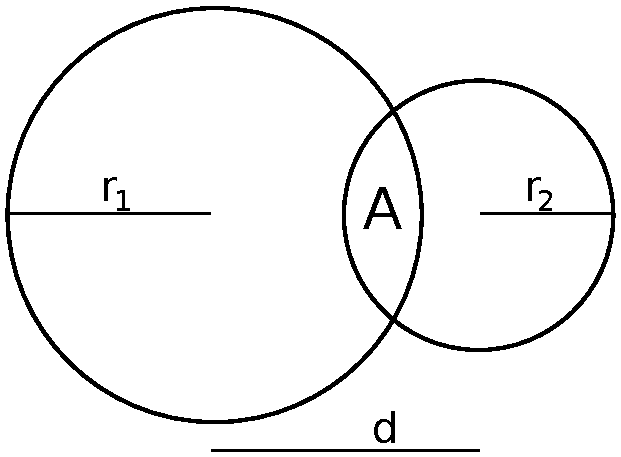
\includegraphics[width=.6\textwidth]{overlapping-area.pdf}
\caption{Overlapping area $A$ of down wind turbine rotor disc with radius $r_2$ and a wake at the down wind turbine with radius $r_1$ caused by an upwind turbine. The distance between the centers of the two circles is denoted $d$.}
\label{fig:overlap}
\end{figure}

We denote the radius of rotor as $r_2$, and the radius of wake at turbine we are looking at as $r_1$. If the distance $d$ between the center of turbine and wake is larger than $(r_1+r_2)$, i.e.,
\begin{equation}
d \geq r_1+r_2
\end{equation}
then we end up no overlap between the turbine and wake. When $d < r_1+r_2$ there begins overlapping, but we need to distinguish between two different cases. If $d$ satisfies the following equation, 
\begin{equation}
r_1-r_2 < d < r_1+r_2
\end{equation}
we have the partially overlap case, where is overlapping area can be found as
\begin{equation}
area = r^2_1 \cos^{-1}\bigg(\frac{r^2_1-r^2_2+d^2}{2dr_1}\bigg)
      +r^2_2 \cos^{-1}\bigg(\frac{r^2_2-r^2_1+d^2}{2dr_2}\bigg)
      -\frac{1}{2}\sqrt{T}
\end{equation}
where $T$ can be calculated as 
\begin{equation}
T = \Big((r_1+r_2)^2-d^2\Big)\Big(d^2-(r_1-r_2)^2 \Big)
\end{equation}
The last case is fairly straightforward, where the turbine is fully covered by the wake, i.e.,
\begin{equation}
	\begin{aligned}
	d \leq r_1-r_2 \\
	area = \pi r^2_2
	\end{aligned}
\end{equation}

\section{Wake deflection due to yaw}
In part b of the exam project you have to include wake deflection due to rotation and yaw. These effects should be excluded in part a. In this case the requirement of overlap is defined as
\begin{equation}
d < r_1+r_2+\delta_\text{rot}+\delta_\text{yaw}
\end{equation}
where $\delta_\text{rot}$ is the wake deflection caused by the rotating blades and $\delta_\text{yaw}$ is the wake deflection due to the yaw angle of the upwind turbine. The expressions for the two deltas are found in the master's thesis of Emil Thøgersen, the wake conference paper, and the report uploaded together with the Nysted wind farm coordinates. 
\end{document}
 